\documentclass[aspectratio=169,11pt]{beamer}

\usepackage[T1]{fontenc}
\usepackage{lmodern}
\usepackage{graphicx}
\usepackage{booktabs}
\usepackage{siunitx}
\usepackage{tikz}
\usetikzlibrary{positioning}
\usepackage{amsmath}
\usepackage{appendixnumberbeamer}
\usepackage{pgfpages}

\ifdefined\shownotes
  \setbeameroption{show notes on second screen=right}
\else
  \setbeameroption{hide notes}
\fi

\definecolor{ink}{HTML}{17243A}
\definecolor{purple}{HTML}{4C2A85}
\definecolor{teal}{HTML}{007C83}
\definecolor{gold}{HTML}{D8A52A}
\definecolor{copper}{HTML}{C7663A}
\definecolor{steel}{HTML}{607D8B}
\definecolor{pale}{HTML}{F3F6F8}
\definecolor{muted}{HTML}{5D6978}
\definecolor{good}{HTML}{2E7D32}
\definecolor{warn}{HTML}{B26A00}

\setbeamertemplate{navigation symbols}{}
\setbeamertemplate{itemize item}{\color{teal}$\blacktriangleright$}
\setbeamertemplate{itemize subitem}{\color{purple}$\bullet$}
\setbeamercolor{normal text}{fg=ink,bg=white}
\setbeamercolor{structure}{fg=purple}
\setbeamercolor{frametitle}{fg=ink,bg=white}
\setbeamercolor{alerted text}{fg=copper}
\setbeamerfont{frametitle}{series=\bfseries,size=\Large}
\setbeamerfont{title}{series=\bfseries,size=\LARGE}
\setbeamerfont{subtitle}{size=\large}

\setbeamertemplate{frametitle}{%
  \vspace{0.12cm}
  \begin{beamercolorbox}[wd=\paperwidth,ht=0.72cm,dp=0.15cm,leftskip=0.48cm,rightskip=0.48cm]{frametitle}
    \usebeamerfont{frametitle}\insertframetitle
  \end{beamercolorbox}
  \vspace{-0.20cm}{\color{teal}\rule{\linewidth}{1.3pt}}
}

\setbeamertemplate{footline}{%
  \leavevmode%
  \hbox{%
    \begin{beamercolorbox}[wd=.74\paperwidth,ht=2.5ex,dp=1.1ex,leftskip=.45cm]{author in head/foot}
      \color{muted}\scriptsize Y. Ashkenazy \(\cdot\) MeVArc 2026
    \end{beamercolorbox}%
    \begin{beamercolorbox}[wd=.24\paperwidth,ht=2.5ex,dp=1.1ex,rightskip=.25cm plus1fil]{page number in head/foot}
      \color{muted}\scriptsize \insertframenumber/\inserttotalframenumber
    \end{beamercolorbox}%
  }%
}

\newcommand{\source}[1]{\vfill{\color{muted}\tiny Source: #1}}
\newcommand{\claim}[1]{%
  \begin{beamercolorbox}[rounded=true,sep=0.18cm,wd=\linewidth]{block body}
    \large\bfseries\color{ink}#1
  \end{beamercolorbox}}
\newcommand{\tagbox}[2]{%
  \tikz[baseline=(n.base)]\node[rounded corners=2pt,fill=#1!13,draw=#1!55,inner xsep=5pt,inner ysep=2pt](n){\color{#1}\bfseries #2};}
\graphicspath{{figures/}}

\title{Does conditioning leave a structural memory?}
\subtitle{From copper evidence to a stainless-steel test}
\author{Yinon Ashkenazy and collaborators}
\institute{The Hebrew University of Jerusalem \quad CERN \quad Consorzio RFX}
\date{MeVArc 2026}

\begin{document}

% 1
{\setbeamertemplate{footline}{}
\begin{frame}[plain]
  \vspace{0.85cm}
  {\color{purple}\rule{2.2cm}{3pt}}\\[0.35cm]
  {\usebeamerfont{title}\color{ink}\inserttitle\par}
  \vspace{0.18cm}
  {\usebeamerfont{subtitle}\color{teal}\insertsubtitle\par}
  \vspace{0.6cm}
  {\large Yinon Ashkenazy and collaborators}\par
  {\normalsize HUJI \(\cdot\) CERN \(\cdot\) Consorzio RFX}\par
  \vfill
  \begin{columns}[c,onlytextwidth]
    \column{0.60\textwidth}
      {\large\bfseries\color{ink}MeVArc 2026}
    \column{0.36\textwidth}
      \raggedleft
      
\includegraphics[height=0.62cm]{huji_logo_long.png}\hspace{0.35cm}
      
\includegraphics[height=0.62cm]{logo_rfx.png}
  \end{columns}
  \note{Open with the operational fact: every high-gradient device must be conditioned, but we still do not know what microscopic variable is being changed. The talk has two halves. First, a completed copper result that gives a structural candidate for that variable. Second, a stainless-steel experiment designed to test whether the mechanism generalizes.}
\end{frame}}

% 2
\begin{frame}{Conditioning works---but what is being conditioned?}
  \begin{columns}[c]
    \column{0.52\textwidth}
      \begin{itemize}\setlength\itemsep{0.65em}
        \item Repeated high-field exposure raises voltage-holding capability.
        \item Conditioning follows \alert{pulse count}, not simply breakdown count.
        \item A local state variable, $E_S$, captures the evolving field tolerance.
      \end{itemize}
    \column{0.44\textwidth}
      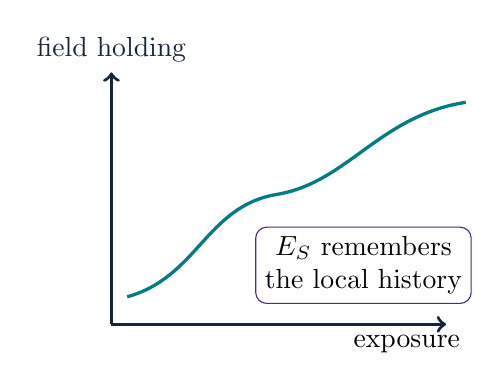
\begin{tikzpicture}[x=1cm,y=1cm]
        \draw[->,very thick,ink] (0,0) -- (4.25,0);
        \node[below] at (3.75,-0.02) {exposure};
        \draw[->,very thick,ink] (0,0) -- (0,3.2) node[above] {field holding};
        \draw[very thick,teal] (0.2,.35) .. controls (1.1,.6) and (1.2,1.5) .. (2.1,1.65)
          .. controls (3.0,1.8) and (3.4,2.65) .. (4.5,2.82);
        \node[fill=white,draw=purple,rounded corners,align=center] at (3.2,.75) {$E_S$ remembers\\the local history};
      \end{tikzpicture}
  \end{columns}
  \claim{The missing link is a measurable material state that survives between pulses.}
  \source{Wuensch et al., Rep. Prog. Phys. (2026); Bjelland et al. (2026).}
  \note{Define $E_S$ operationally: the local field level to which a surface element has conditioned in the Monte Carlo description. Emphasize that it is phenomenological; the model did not identify its microscopic carrier. The question for this talk is whether the subsurface dislocation population can provide that memory.}
\end{frame}

% 3
\begin{frame}{Dislocations are a plausible carrier of that memory}
  \begin{columns}[c]
    \column{0.58\textwidth}
      \begin{itemize}\setlength\itemsep{0.55em}
        \item Breakdown statistics and material trends track barriers to dislocation motion.
        \item The MDDF model treats initiation as a collective dislocation instability.
        \item Local TEM finds a ${\sim}\SI{200}{nm}$ dislocation-denuded layer in conditioned hard Cu.
      \end{itemize}
    \column{0.38\textwidth}
      \begin{beamercolorbox}[rounded=true,sep=.35cm]{block body}
        \centering
        \textbf{Maxwell stress}\\[0.15cm]
        $\displaystyle \sigma_M=\frac{\varepsilon_0 E^2}{2}$\\[0.28cm]
        at $\SI{80}{MV/m}$: \alert{$\SI{0.028}{MPa}$}\\[0.2cm]
        \scriptsize tiny per pulse, repeated ${\sim}10^9$ times
      \end{beamercolorbox}
  \end{columns}
  \claim{The hypothesis is cumulative, field-driven plastic rearrangement below macroscopic yield.}
  \source{Engelberg et al., PRL 2018 / PRAB 2019; Jacewicz et al., PRAB 2025.}
  \note{Do not claim ordinary fatigue equivalence: the Maxwell stress is about three orders below annealed-copper yield. The relevance of very-high-cycle fatigue is conceptual---many sub-yield cycles can accumulate irreversible rearrangement. The MDDF model is valuable because it is threshold-free and connects collective fluctuations to the steep field dependence of breakdown.}
\end{frame}

% 4
\begin{frame}{One cathode turns field exposure into a controlled coordinate}
  \begin{columns}[c]
    \column{0.57\textwidth}
      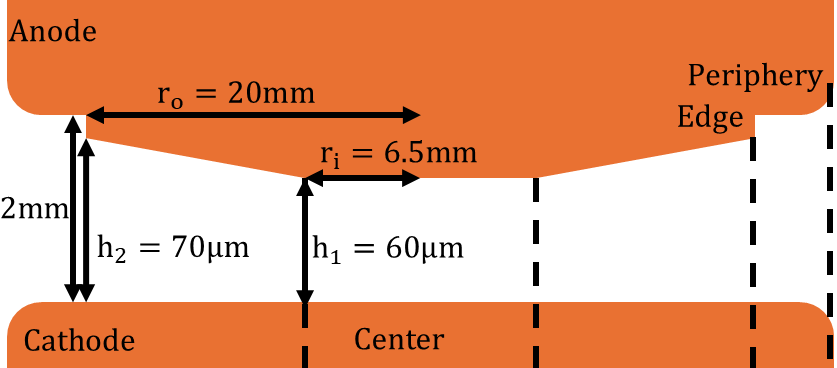
\includegraphics[width=\linewidth]{electrode_geometry.png}
    \column{0.39\textwidth}
      \begin{itemize}\setlength\itemsep{0.48em}
        \item OFE Cu, pulsed DC
        \item $\SI{1}{\micro s}$ pulses at $\SI{1}{kHz}$
        \item Peak field ${\sim}\SI{80}{MV/m}$
        \item Nine EBSD regions: center, edge, periphery, and external reference
      \end{itemize}
  \end{columns}
  \claim{The spatial gradient supplies internal controls on the same specimen.}
  \source{Ashkenazy et al., submitted to PRAB (2026); geometry from Bjelland et al.}
  \note{This geometry is the core experimental design. The flat center is at the maximum field; the sloped gap creates a continuous radial decay; beyond the anode radius the field is below about 2.5 MV/m. Comparing positions on one cathode reduces sensitivity to cathode-to-cathode preparation differences. A separate identically treated, unexposed cathode gives an external reference.}
\end{frame}

% 5
\begin{frame}{EBSD maps plastic activity far from breakdown craters}
  \begin{columns}[c]
    \column{0.47\textwidth}
      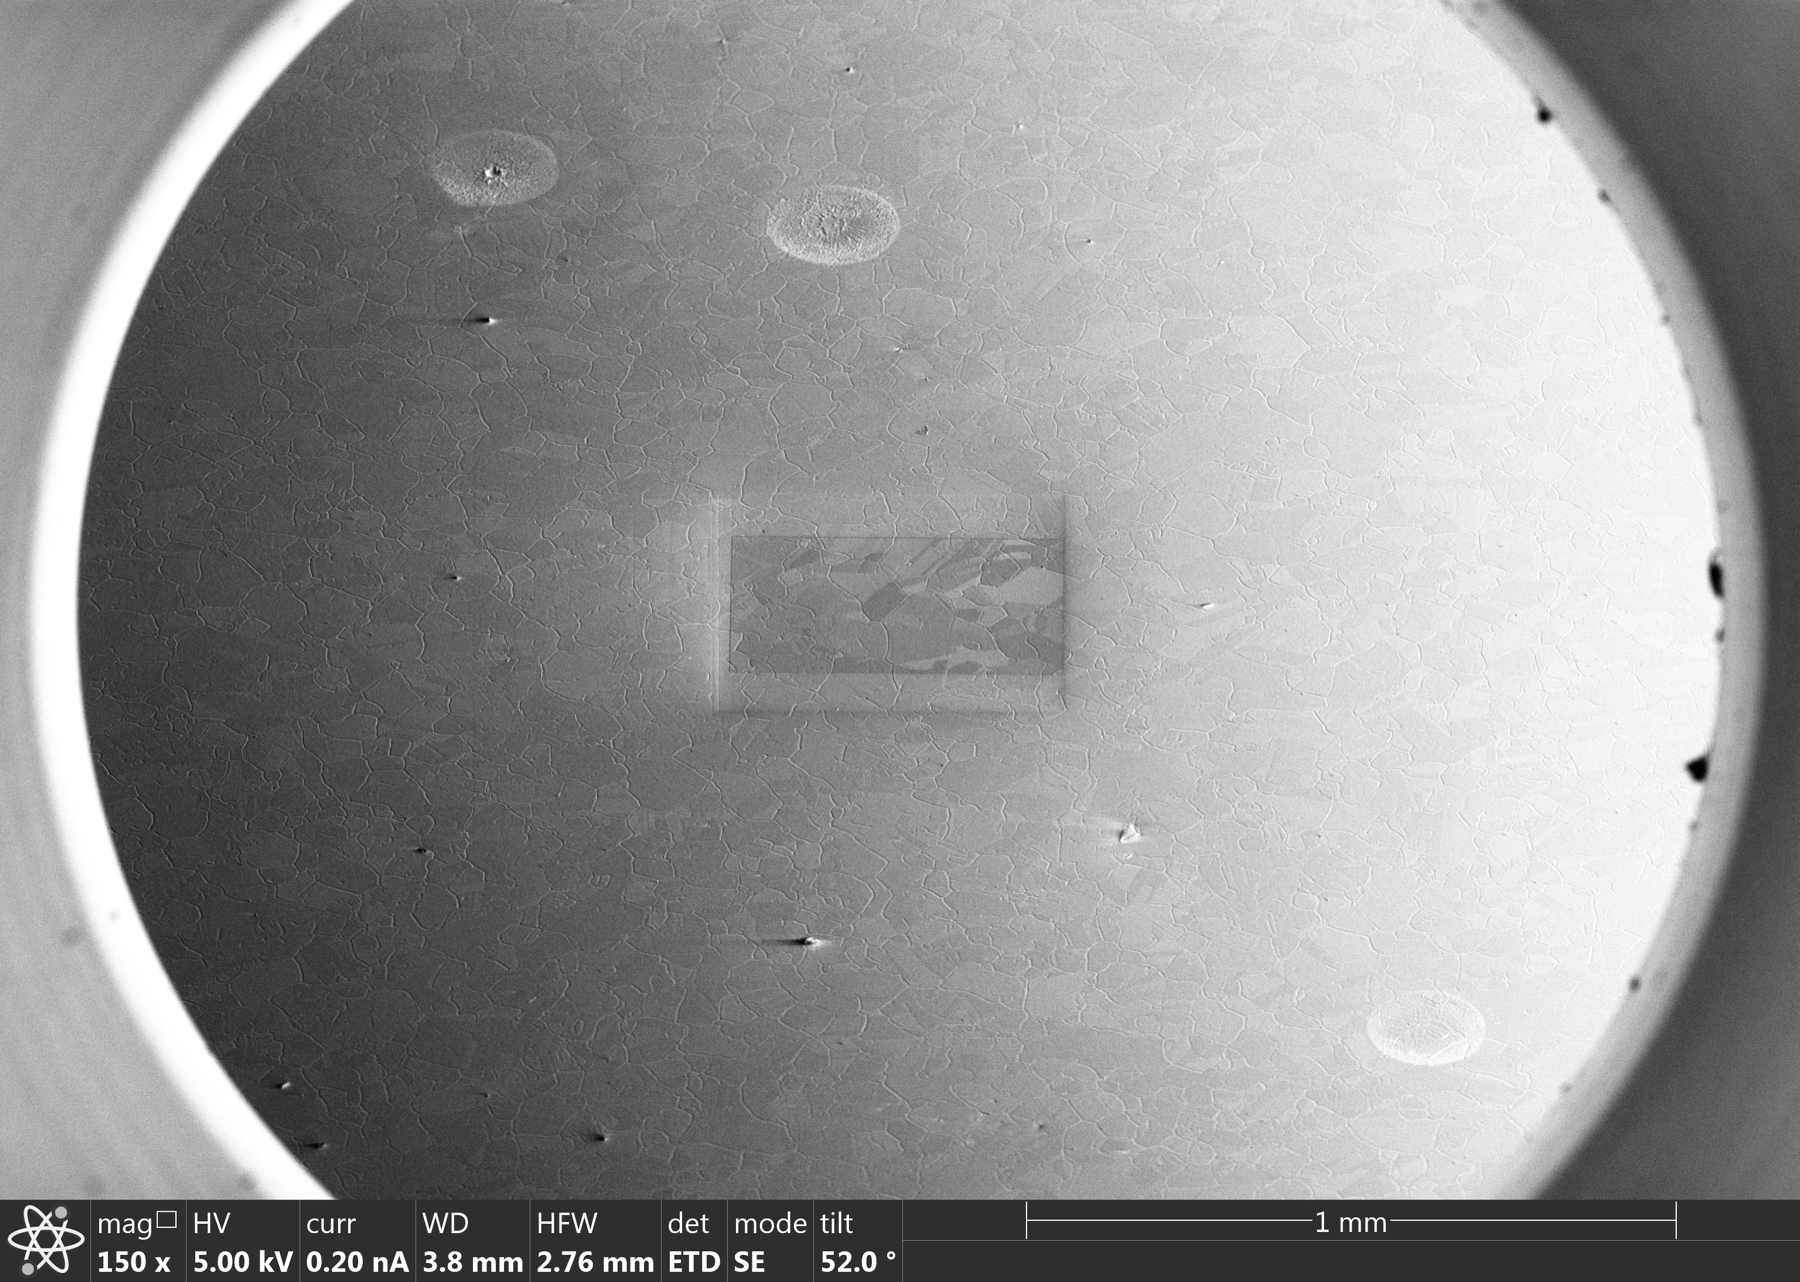
\includegraphics[width=\linewidth]{sem_lowmag.png}
      \vspace{-0.15cm}
      {\scriptsize Cleaned ROI is hundreds of microns from visible craters.}
    \column{0.49\textwidth}
      \begin{itemize}\setlength\itemsep{0.45em}
        \item $\SI{500}{\micro m}$-wide maps; $\SI{3}{\micro m}$ step
        \item ${\sim}24{,}000$ indexed points per ROI
        \item LAM, KAM, and LOS probe intragrain orientation gradients
        \item Misorientation is a proxy for geometrically necessary dislocation density
      \end{itemize}
  \end{columns}
  \claim{This separates cumulative field exposure from the local aftermath of an arc.}
  \source{cond26 manuscript, experimental methods.}
  \note{Explain the cleaning and selection briefly: a shallow FIB removal of oxide, less than 10 nm by AFM, followed by EBSD. All regions were deliberately chosen away from craters. LAM is the primary visual metric; two other definitions are used to check that the result is not an artifact of one analysis choice.}
\end{frame}

% 6
\begin{frame}{High-field copper contains more intragrain curvature}
  \begin{columns}[T]
    \column{0.49\textwidth}
      \centering
      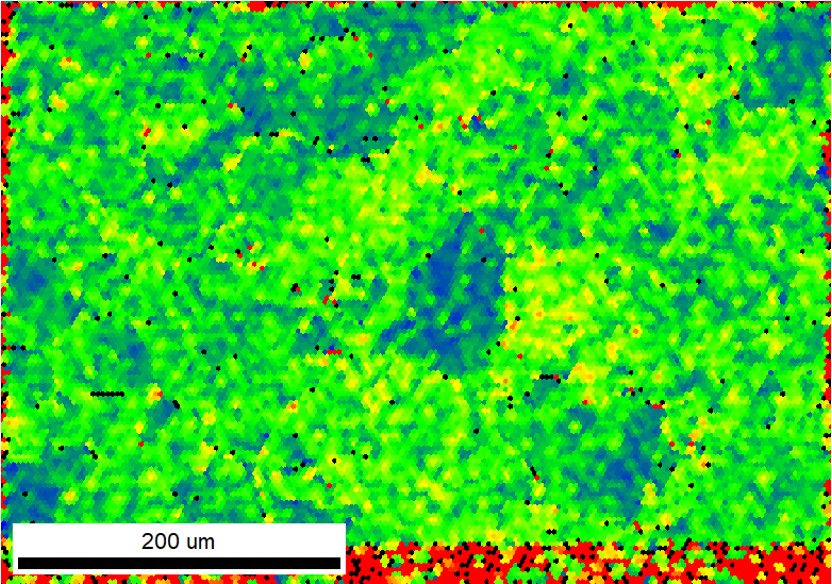
\includegraphics[width=\linewidth,height=4.8cm,keepaspectratio]{lam_fe_center.png}\\[-1mm]
      \tagbox{copper}{Field-exposed center}
    \column{0.49\textwidth}
      \centering
      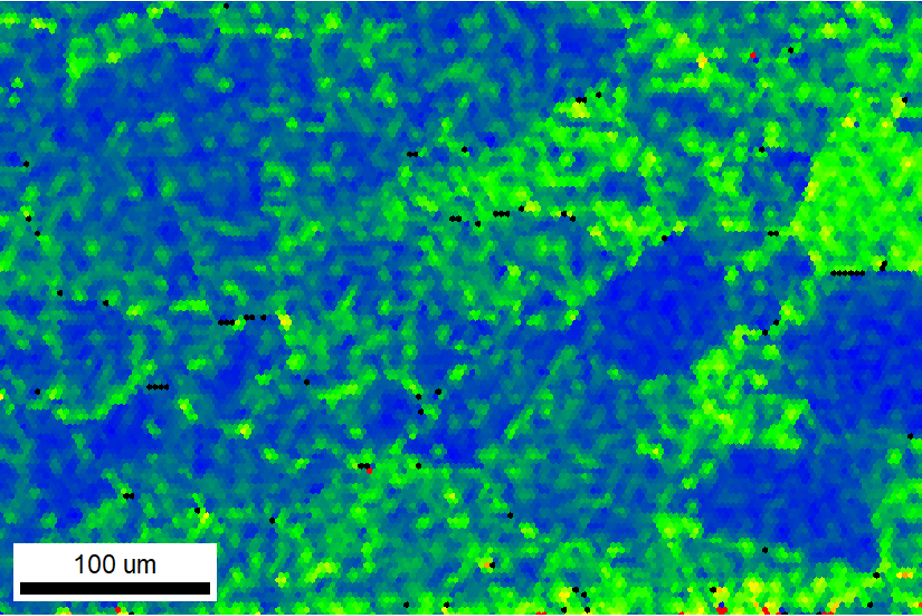
\includegraphics[width=\linewidth,height=4.8cm,keepaspectratio]{lam_ref_edge.png}\\[-1mm]
      \tagbox{teal}{Unexposed reference}
  \end{columns}
  \source{Ashkenazy et al., submitted to PRAB (2026). Same LAM color scale.}
  \note{Invite the audience to look at the spatial texture, not just the color average. The field-exposed region carries more high-misorientation structure within grains. State that the comparison shown is representative, while the quantitative conclusion is based on all nine ROIs.}
\end{frame}

% 7
\begin{frame}{The signal separates into three exposure tiers}
  \begin{columns}[c]
    \column{0.62\textwidth}
      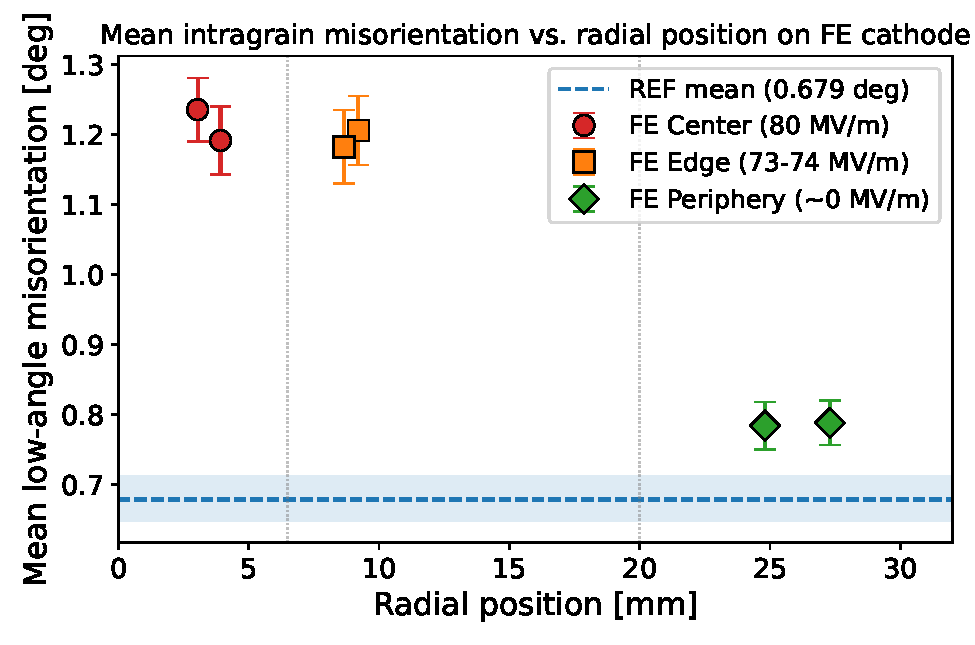
\includegraphics[width=0.96\linewidth]{mean_vs_radius.pdf}
    \column{0.34\textwidth}
      \begin{itemize}\setlength\itemsep{0.55em}
        \item Center and edge: ${\sim}\ang{1.2}$
        \item External reference: ${\sim}\ang{0.68}$
        \item High field is \alert{${\sim}75\%$ higher}
        \item Grain size does not follow this hierarchy
      \end{itemize}
  \end{columns}
  \claim{The ordering follows field history, not merely sample position or grain size.}
  \source{Ashkenazy et al., submitted to PRAB (2026).}
  \note{Walk through the tiers: high-field center and edge are similar; the field-exposed periphery is intermediate; unexposed references are lowest. The periphery is useful because it shared machining, heat treatment, mounting, vacuum, and handling with the high-field regions but experienced negligible field. Be explicit that the 75 percent value characterizes this cathode and history, not a universal material constant.}
\end{frame}

% 8
\begin{frame}{Field exposure populates a high-misorientation tail}
  \begin{columns}[c]
    \column{0.61\textwidth}
      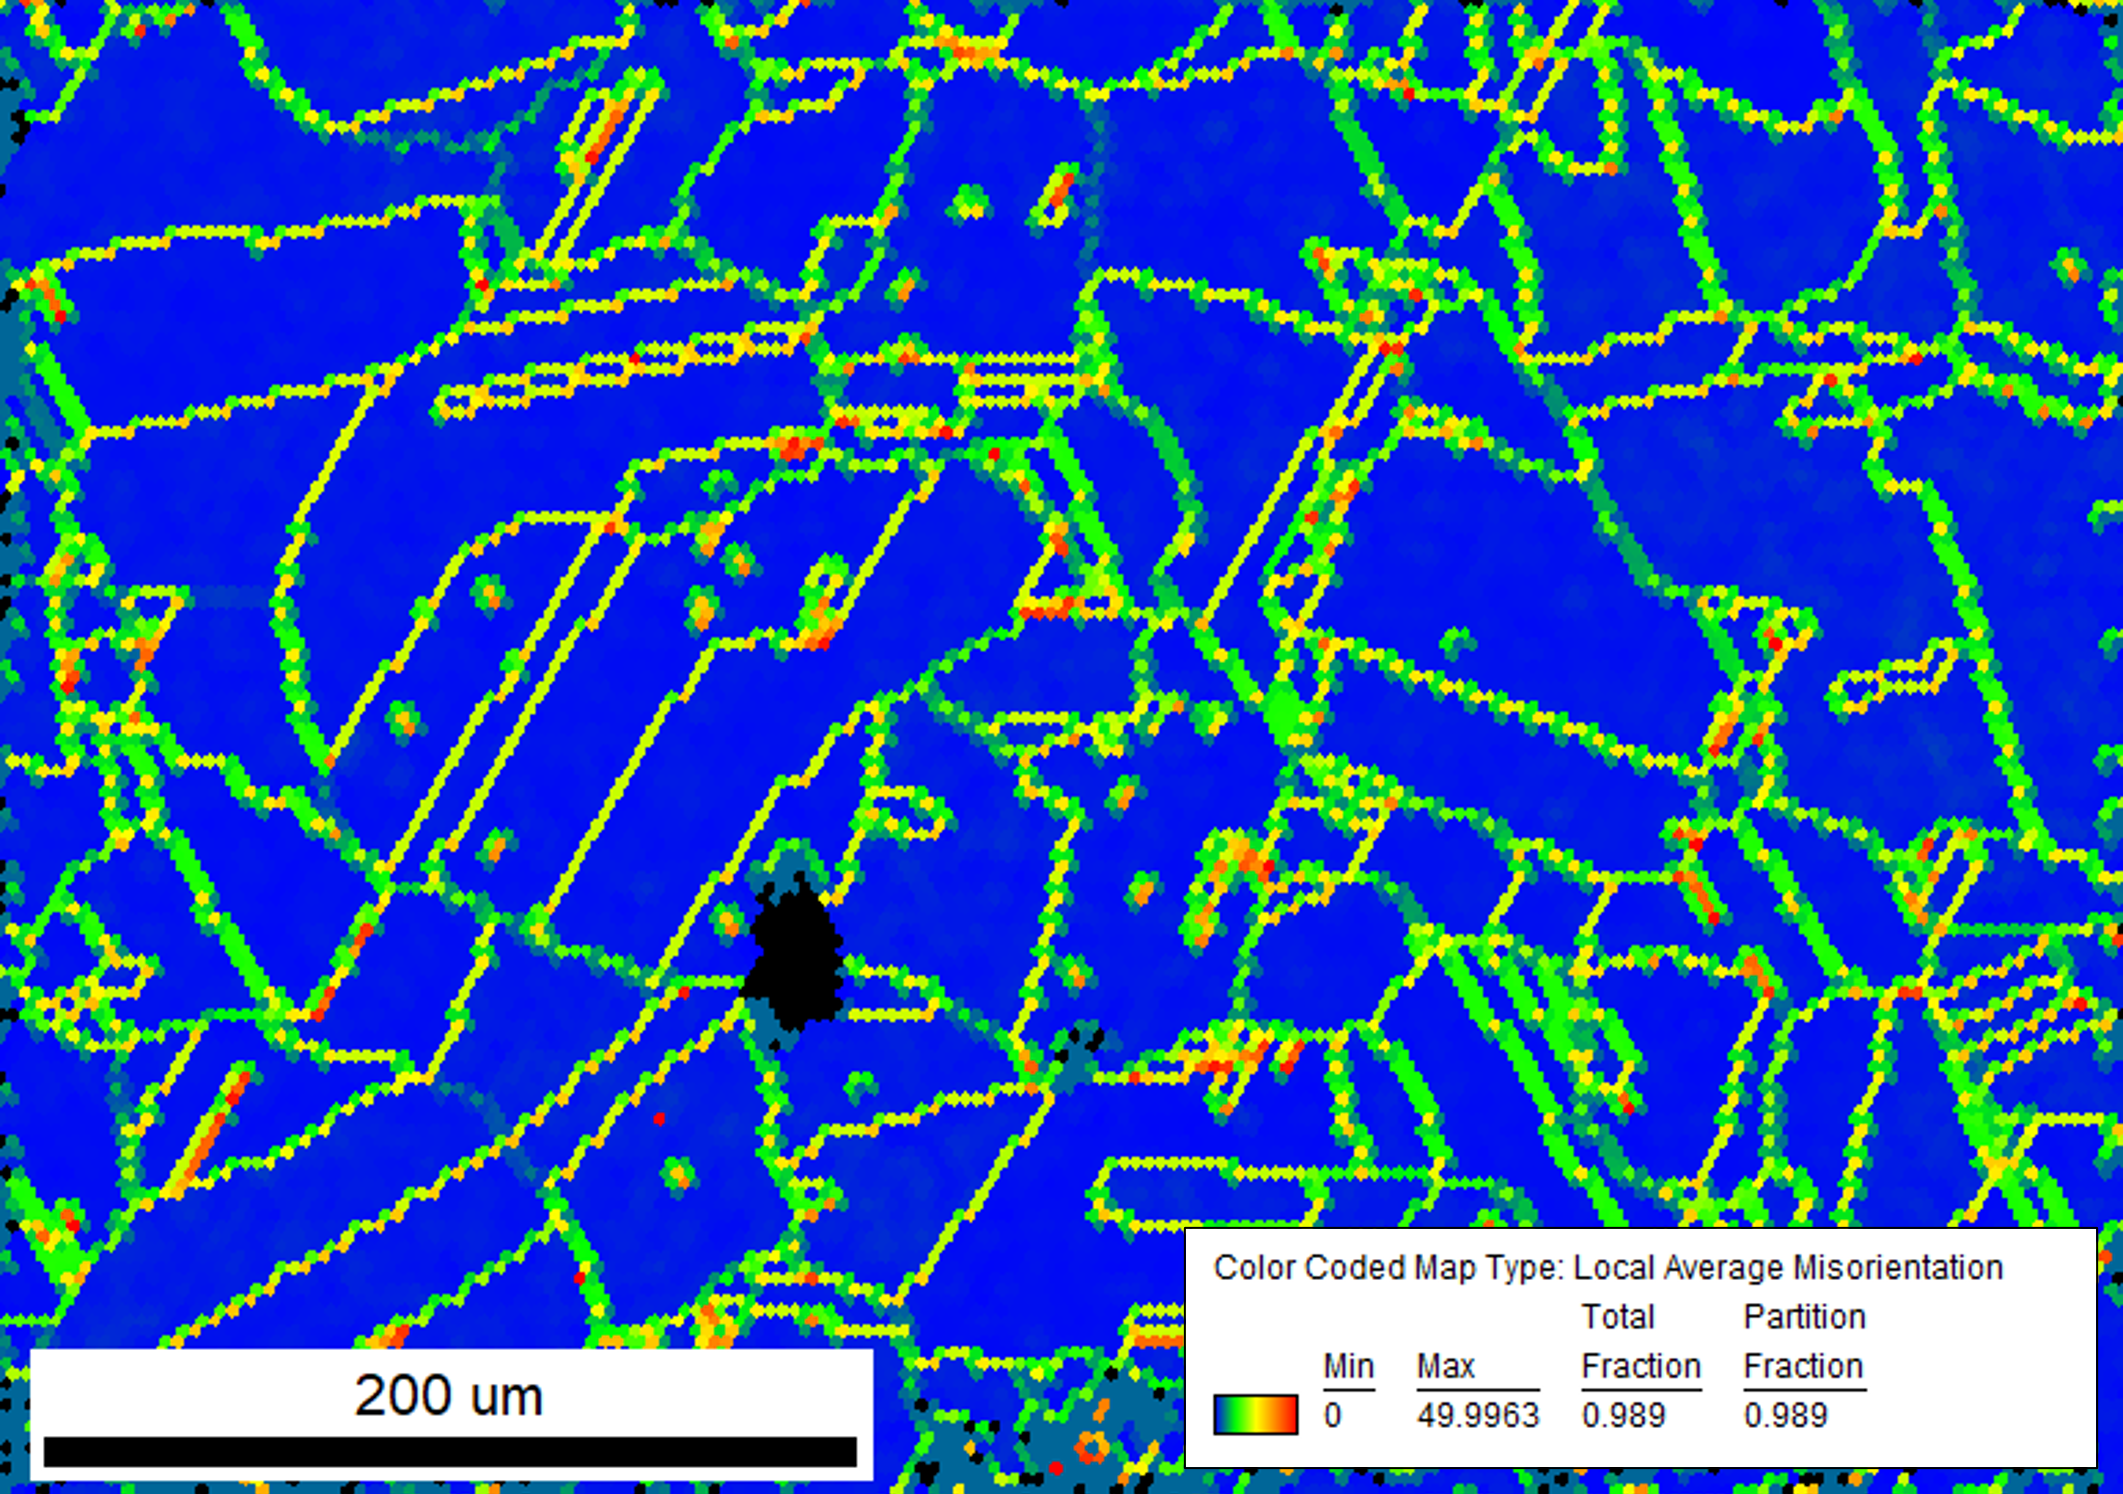
\includegraphics[width=\linewidth,height=4.75cm,keepaspectratio]{lam_widescale.png}
    \column{0.35\textwidth}
      \begin{beamercolorbox}[rounded=true,sep=.28cm]{block body}
        \centering
        \textbf{LAM tail above $\ang{2}$}\\[0.2cm]
        \alert{${\sim}0.14$} field-exposed\\
        ${\sim}0.016$ reference\\[0.15cm]
        \textbf{${\sim}8\times$ increase}
      \end{beamercolorbox}
      \vspace{0.35cm}
      {\small All center/edge distributions differ from unexposed references: $D_{KS}>0.25$.}
  \end{columns}
  \claim{Field exposure redistributes orientation; it is not a uniform offset.}
  \source{cond26 manuscript, distribution analysis.}
  \note{The mean is not the whole story. The distribution broadens strongly and acquires a long tail. Mention that LAM, KAM, and LOS reproduce the ordering, and that KS, chi-squared, and Anderson--Darling tests all distinguish the high-field and unexposed distributions. Avoid overselling pixel-level independence; the statistics demonstrate robust distribution separation across the maps.}
\end{frame}

% 9
\begin{frame}{A material state now shadows the conditioning state $E_S$}
  \centering
  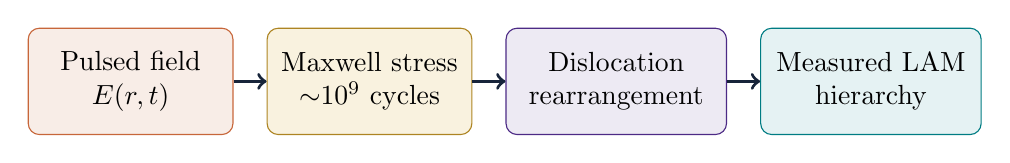
\begin{tikzpicture}[node distance=0.42cm]
    \node[draw=copper,fill=copper!12,rounded corners,minimum width=2.6cm,minimum height=1.35cm,align=center] (a) {Pulsed field\\$E(r,t)$};
    \node[draw=gold!80!black,fill=gold!15,rounded corners,minimum width=2.6cm,minimum height=1.35cm,align=center,right=of a] (b) {Maxwell stress\\${\sim}10^9$ cycles};
    \node[draw=purple,fill=purple!10,rounded corners,minimum width=2.8cm,minimum height=1.35cm,align=center,right=of b] (c) {Dislocation\\rearrangement};
    \node[draw=teal,fill=teal!10,rounded corners,minimum width=2.8cm,minimum height=1.35cm,align=center,right=of c] (d) {Measured LAM\\hierarchy};
    \draw[->,very thick,ink] (a)--(b); \draw[->,very thick,ink] (b)--(c); \draw[->,very thick,ink] (c)--(d);
  \end{tikzpicture}
  \vspace{0.65cm}
  \begin{columns}[c]
    \column{0.47\textwidth}
      \centering\tagbox{purple}{$E_S$: phenomenological memory}
    \column{0.06\textwidth}\centering{$\Longleftrightarrow$}
    \column{0.47\textwidth}
      \centering\tagbox{teal}{Misorientation: structural memory}
  \end{columns}
  \vspace{0.45cm}
  \claim{The evolving subsurface dislocation population is a candidate physical basis for $E_S$.}
  \note{Use candidate, not identification. The spatial ordering matches, but a point-by-point quantitative correlation with the simulated $E_S(r)$ still requires more radial positions and finer EBSD. The result is nevertheless the first large-area comparison that connects conditioned and unconditioned regions through a dislocation-sensitive structural observable.}
\end{frame}

% 10
\begin{frame}{Copper establishes the effect; it does not establish universality}
  \begin{columns}[T]
    \column{0.48\textwidth}
      \tagbox{good}{What is established}
      \begin{itemize}\setlength\itemsep{0.38em}
        \item Large-area structural difference
        \item Three independent metrics
        \item Internal and external controls
        \item Spatial ordering consistent with $E_S$
      \end{itemize}
    \column{0.48\textwidth}
      \tagbox{warn}{What remains open}
      \begin{itemize}\setlength\itemsep{0.38em}
        \item Full depth profile
        \item Grain-orientation dependence
        \item More conditioned cathodes
        \item Cross-material generality
      \end{itemize}
  \end{columns}
  \claim{A stronger test changes both the material and the loading history.}
  \note{This is the transition slide. Acknowledge the single conditioned cathode and single external reference. Depth is especially important because TEM reports depletion in the top 200 nm while EBSD reports accumulated curvature over a larger interaction volume. These may be parts of one redistribution profile. The stainless-steel collaboration supplies an orthogonal test rather than a simple replication.}
\end{frame}

% 11
\begin{frame}{Stainless steel is a deliberately difficult test}
  \begin{columns}[T]
    \column{0.46\textwidth}
      \begin{beamercolorbox}[rounded=true,sep=.30cm]{block body}
        \centering\Large\bfseries\color{copper} Copper\\[0.2cm]
        \normalsize FCC, higher SFE\\
        easier cross-slip\\
        pulsed DC loading\\
        ${\sim}10^9$ cycles
      \end{beamercolorbox}
    \column{0.08\textwidth}\centering\vspace{1.25cm}{\Huge$\neq$}
    \column{0.46\textwidth}
      \begin{beamercolorbox}[rounded=true,sep=.30cm]{block body}
        \centering\Large\bfseries\color{steel} AISI 304 SS\\[0.2cm]
        \normalsize metastable austenite, lower SFE\\
        planar slip / possible twinning\\
        continuous DC exposure\\
        possible $\gamma\!\to\!\varepsilon\!\to\!\alpha'$ transformation
      \end{beamercolorbox}
  \end{columns}
  \vspace{0.4cm}
  \claim{A correlated SS response would support a mechanism broader than one alloy or pulse protocol.}
  \note{Clarify that the drawing specifies AISI 304; the exact sub-grade and composition certificate remain outstanding. Stainless steel changes stacking-fault energy, dislocation mobility, and introduces metastable phase transformations. Continuous DC is creep-like rather than the copper experiment's cyclic loading. Similar spatial behavior under these differences would be powerful; different behavior would also be physically informative.}
\end{frame}

% 12
\begin{frame}{The RFX electrodes provide a second field gradient}
  \begin{columns}[c]
    \column{0.35\textwidth}
      \centering
      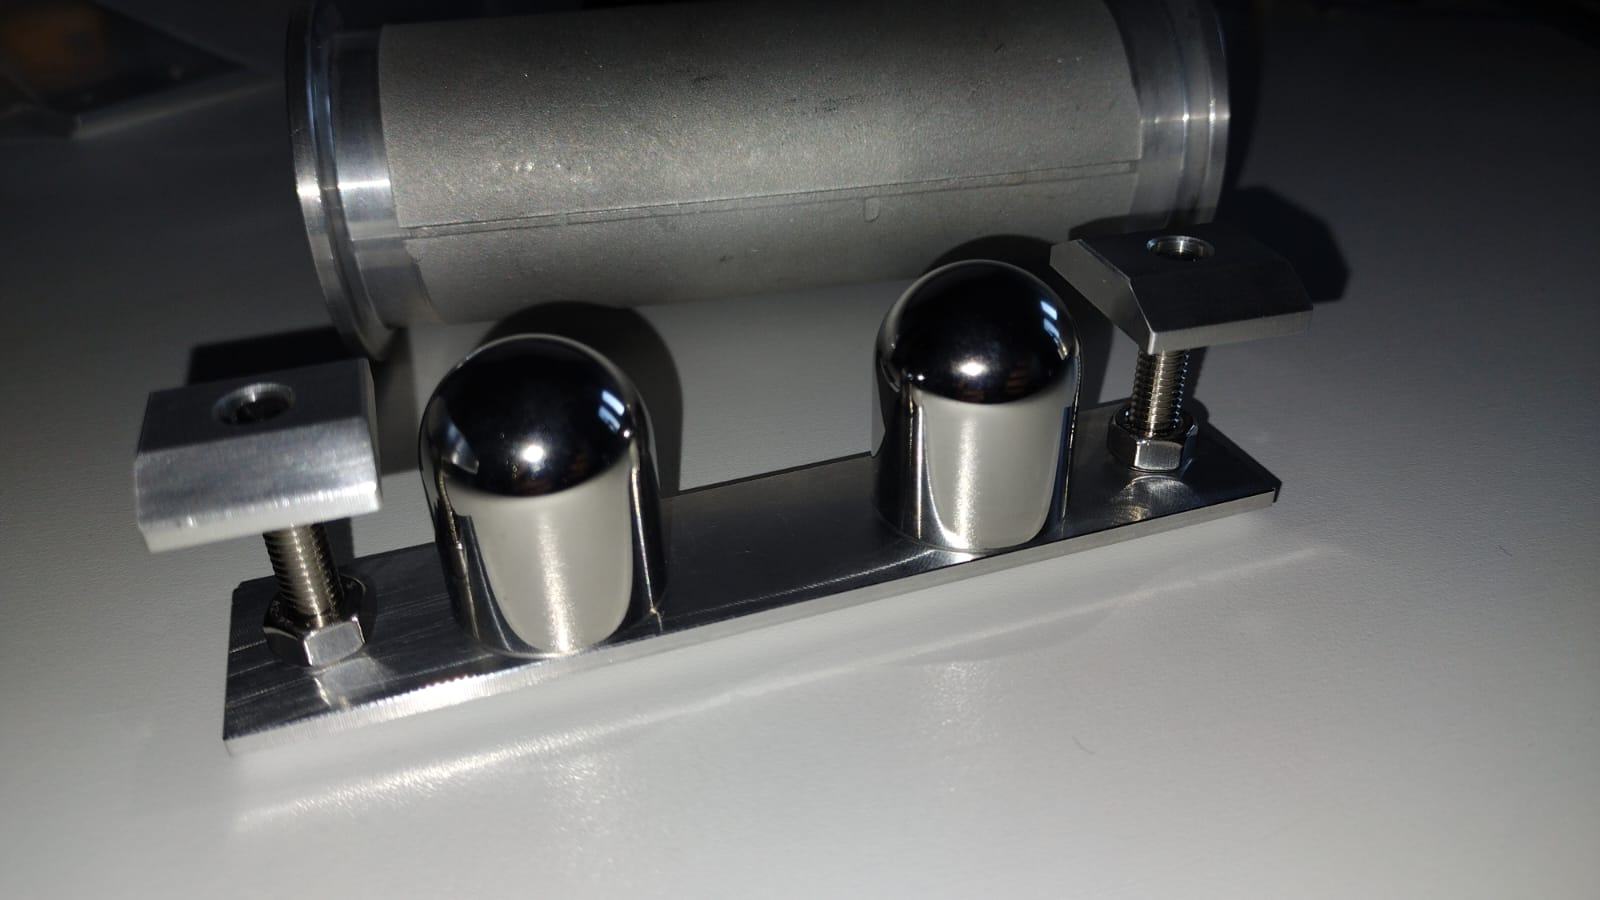
\includegraphics[width=.94\linewidth,height=4.7cm,keepaspectratio]{electrode_photo.jpg}\\[-1mm]
      {\scriptsize HVPTF sphere--plane assembly}
    \column{0.27\textwidth}
      \centering
      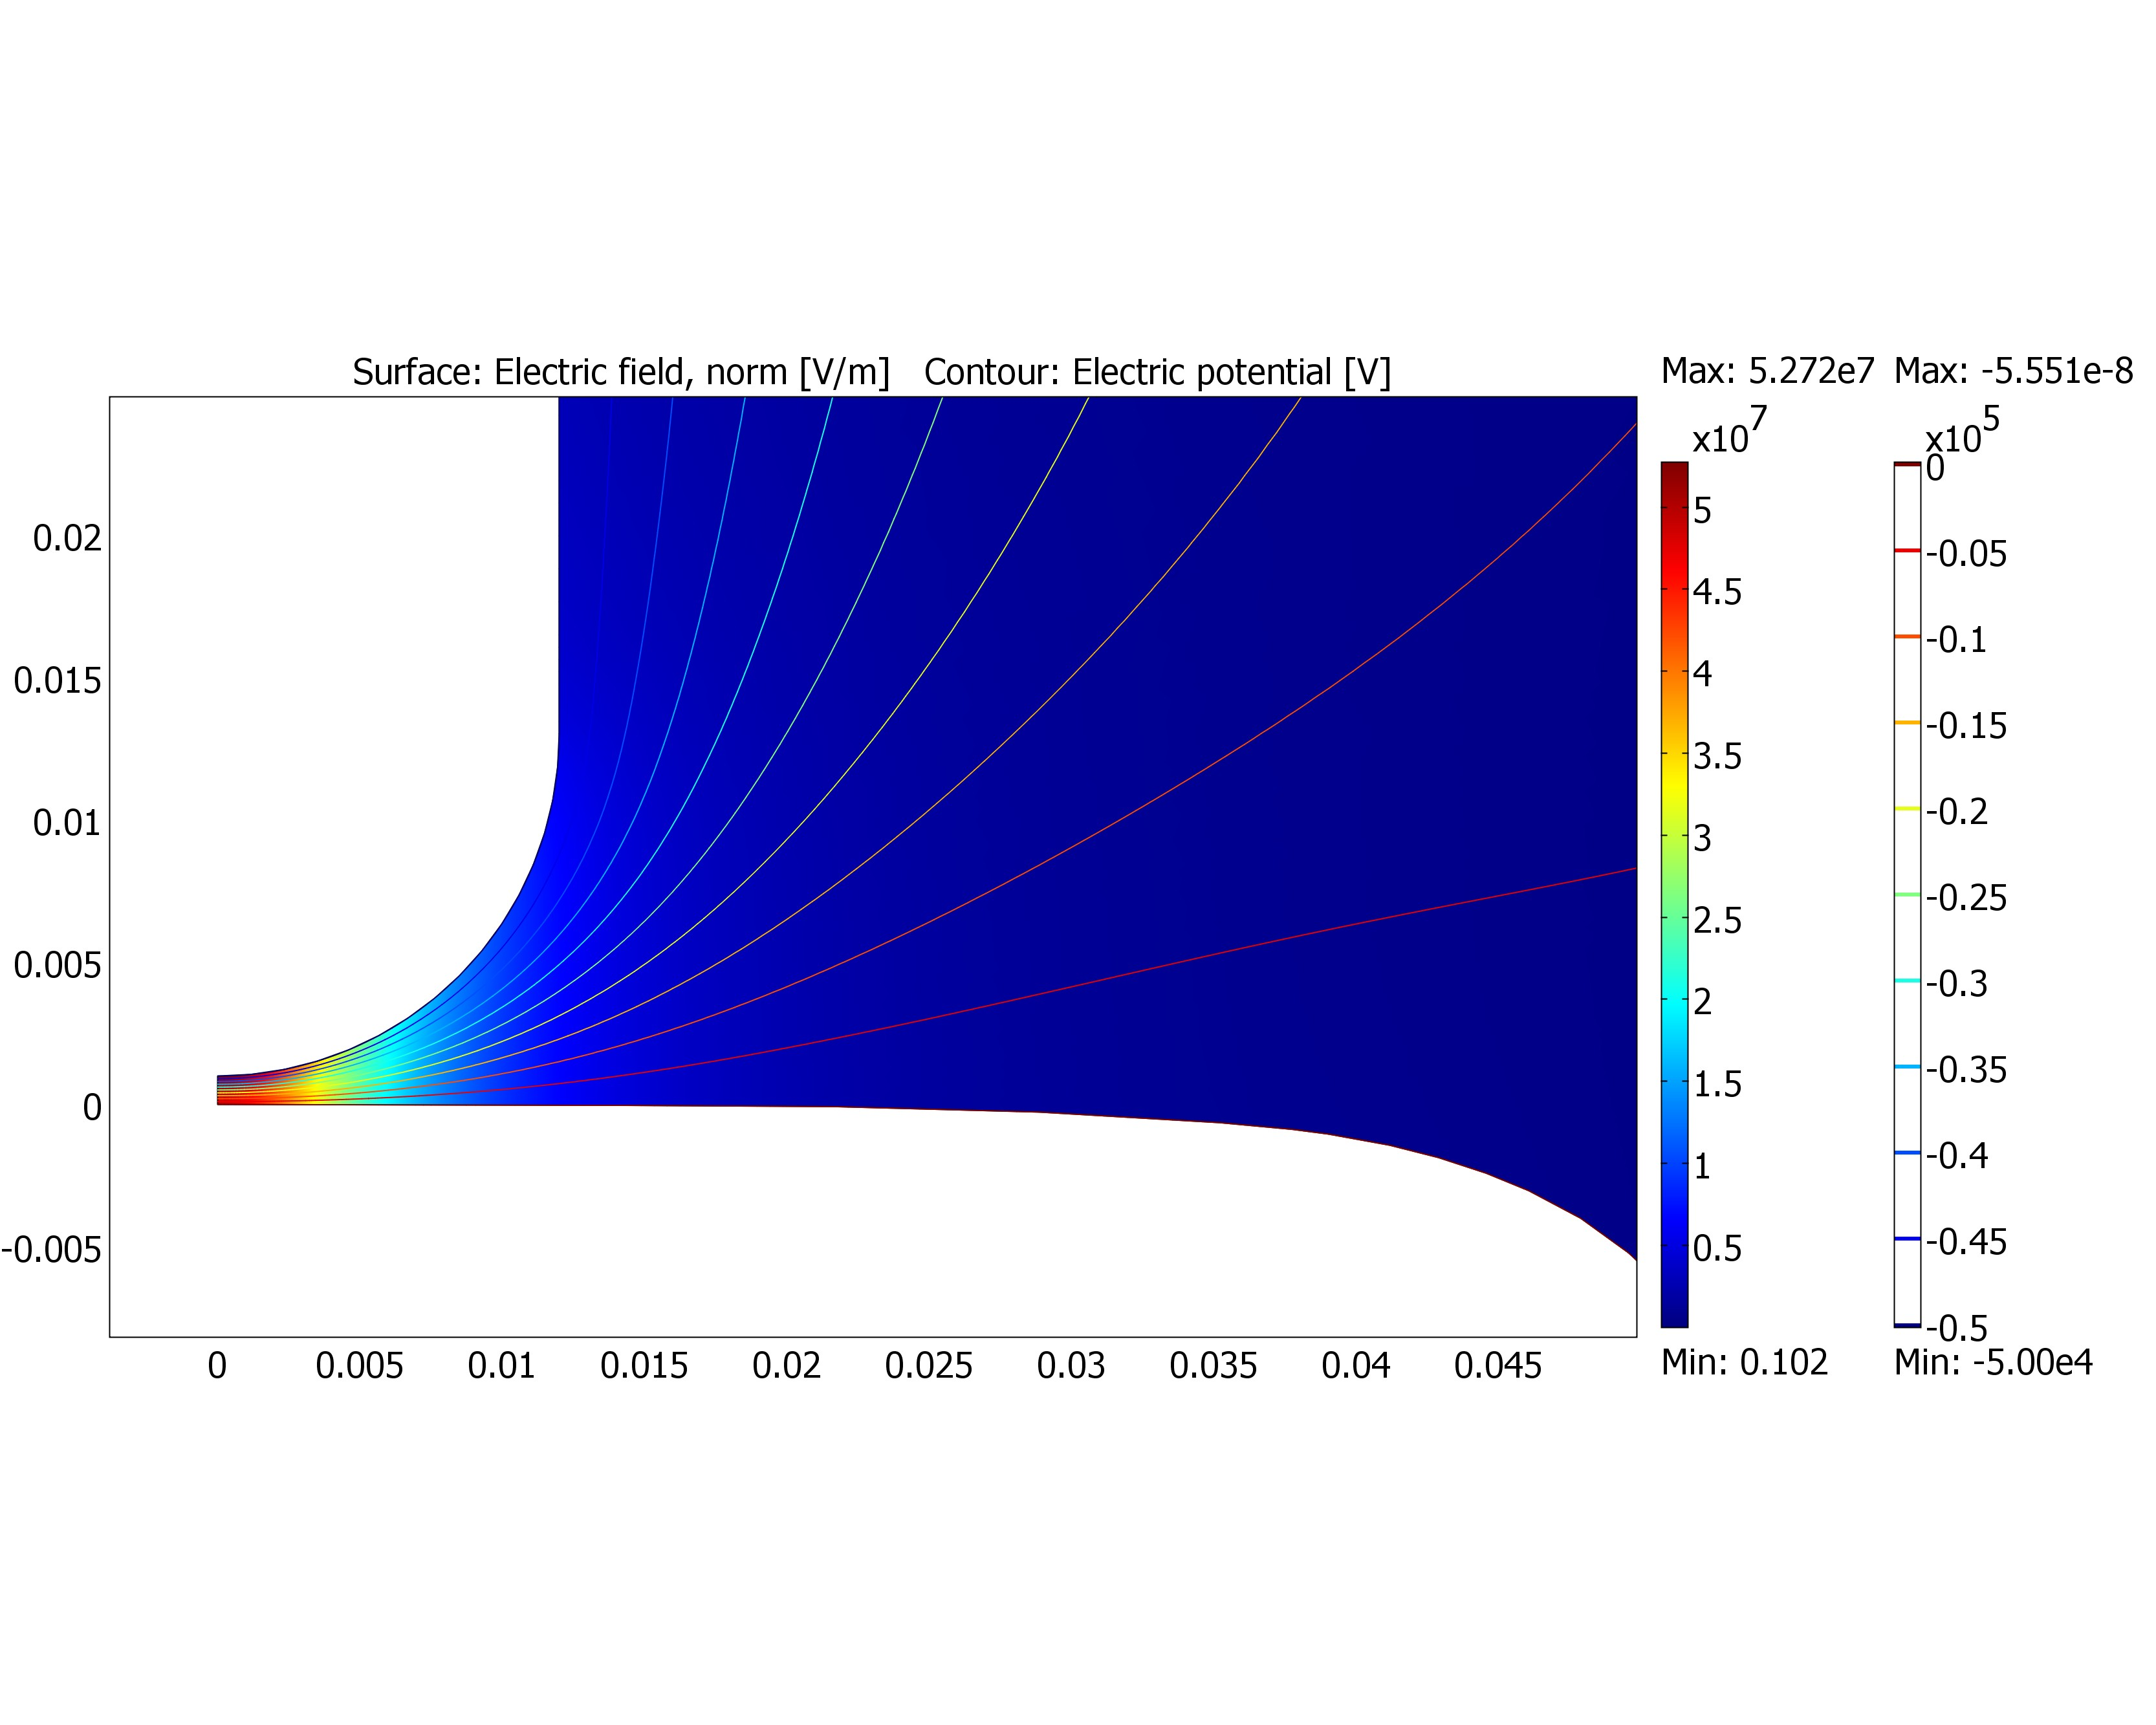
\includegraphics[width=.95\linewidth,height=4.7cm,keepaspectratio]{efield_map.jpg}\\[-1mm]
      {\scriptsize Simulated field map}
    \column{0.34\textwidth}
      \begin{itemize}\setlength\itemsep{0.38em}
        \item $\varnothing\SI{24}{mm}$ hemispherical cathode
        \item $\SI{1}{mm}$ gap
        \item two exposed electrodes
        \item $\geq\SI{100}{h}$ at $60$--$\SI{80}{MV/m}$
        \item two batch-matched references
      \end{itemize}
  \end{columns}
  \claim{Apex-to-periphery variation enables an internal field-correlation test.}
  \source{Consorzio RFX electrode drawing and electrostatic simulation; RFX project status, July 2026.}
  \note{The RFX High Voltage Padova Test Facility operates a long-gap DC system. The local field is highest at the hemisphere apex and falls toward the periphery. That gradient is crucial because it can distinguish a conditioning response from sample-to-sample electropolishing differences. Conditioning histories and a numerical field-versus-angle vector are still requested; do not imply that the full exposure map is already available.}
\end{frame}

% 13
\begin{frame}{The first SEM survey reveals a new surface signature}
  \begin{columns}[c]
    \column{0.69\textwidth}
      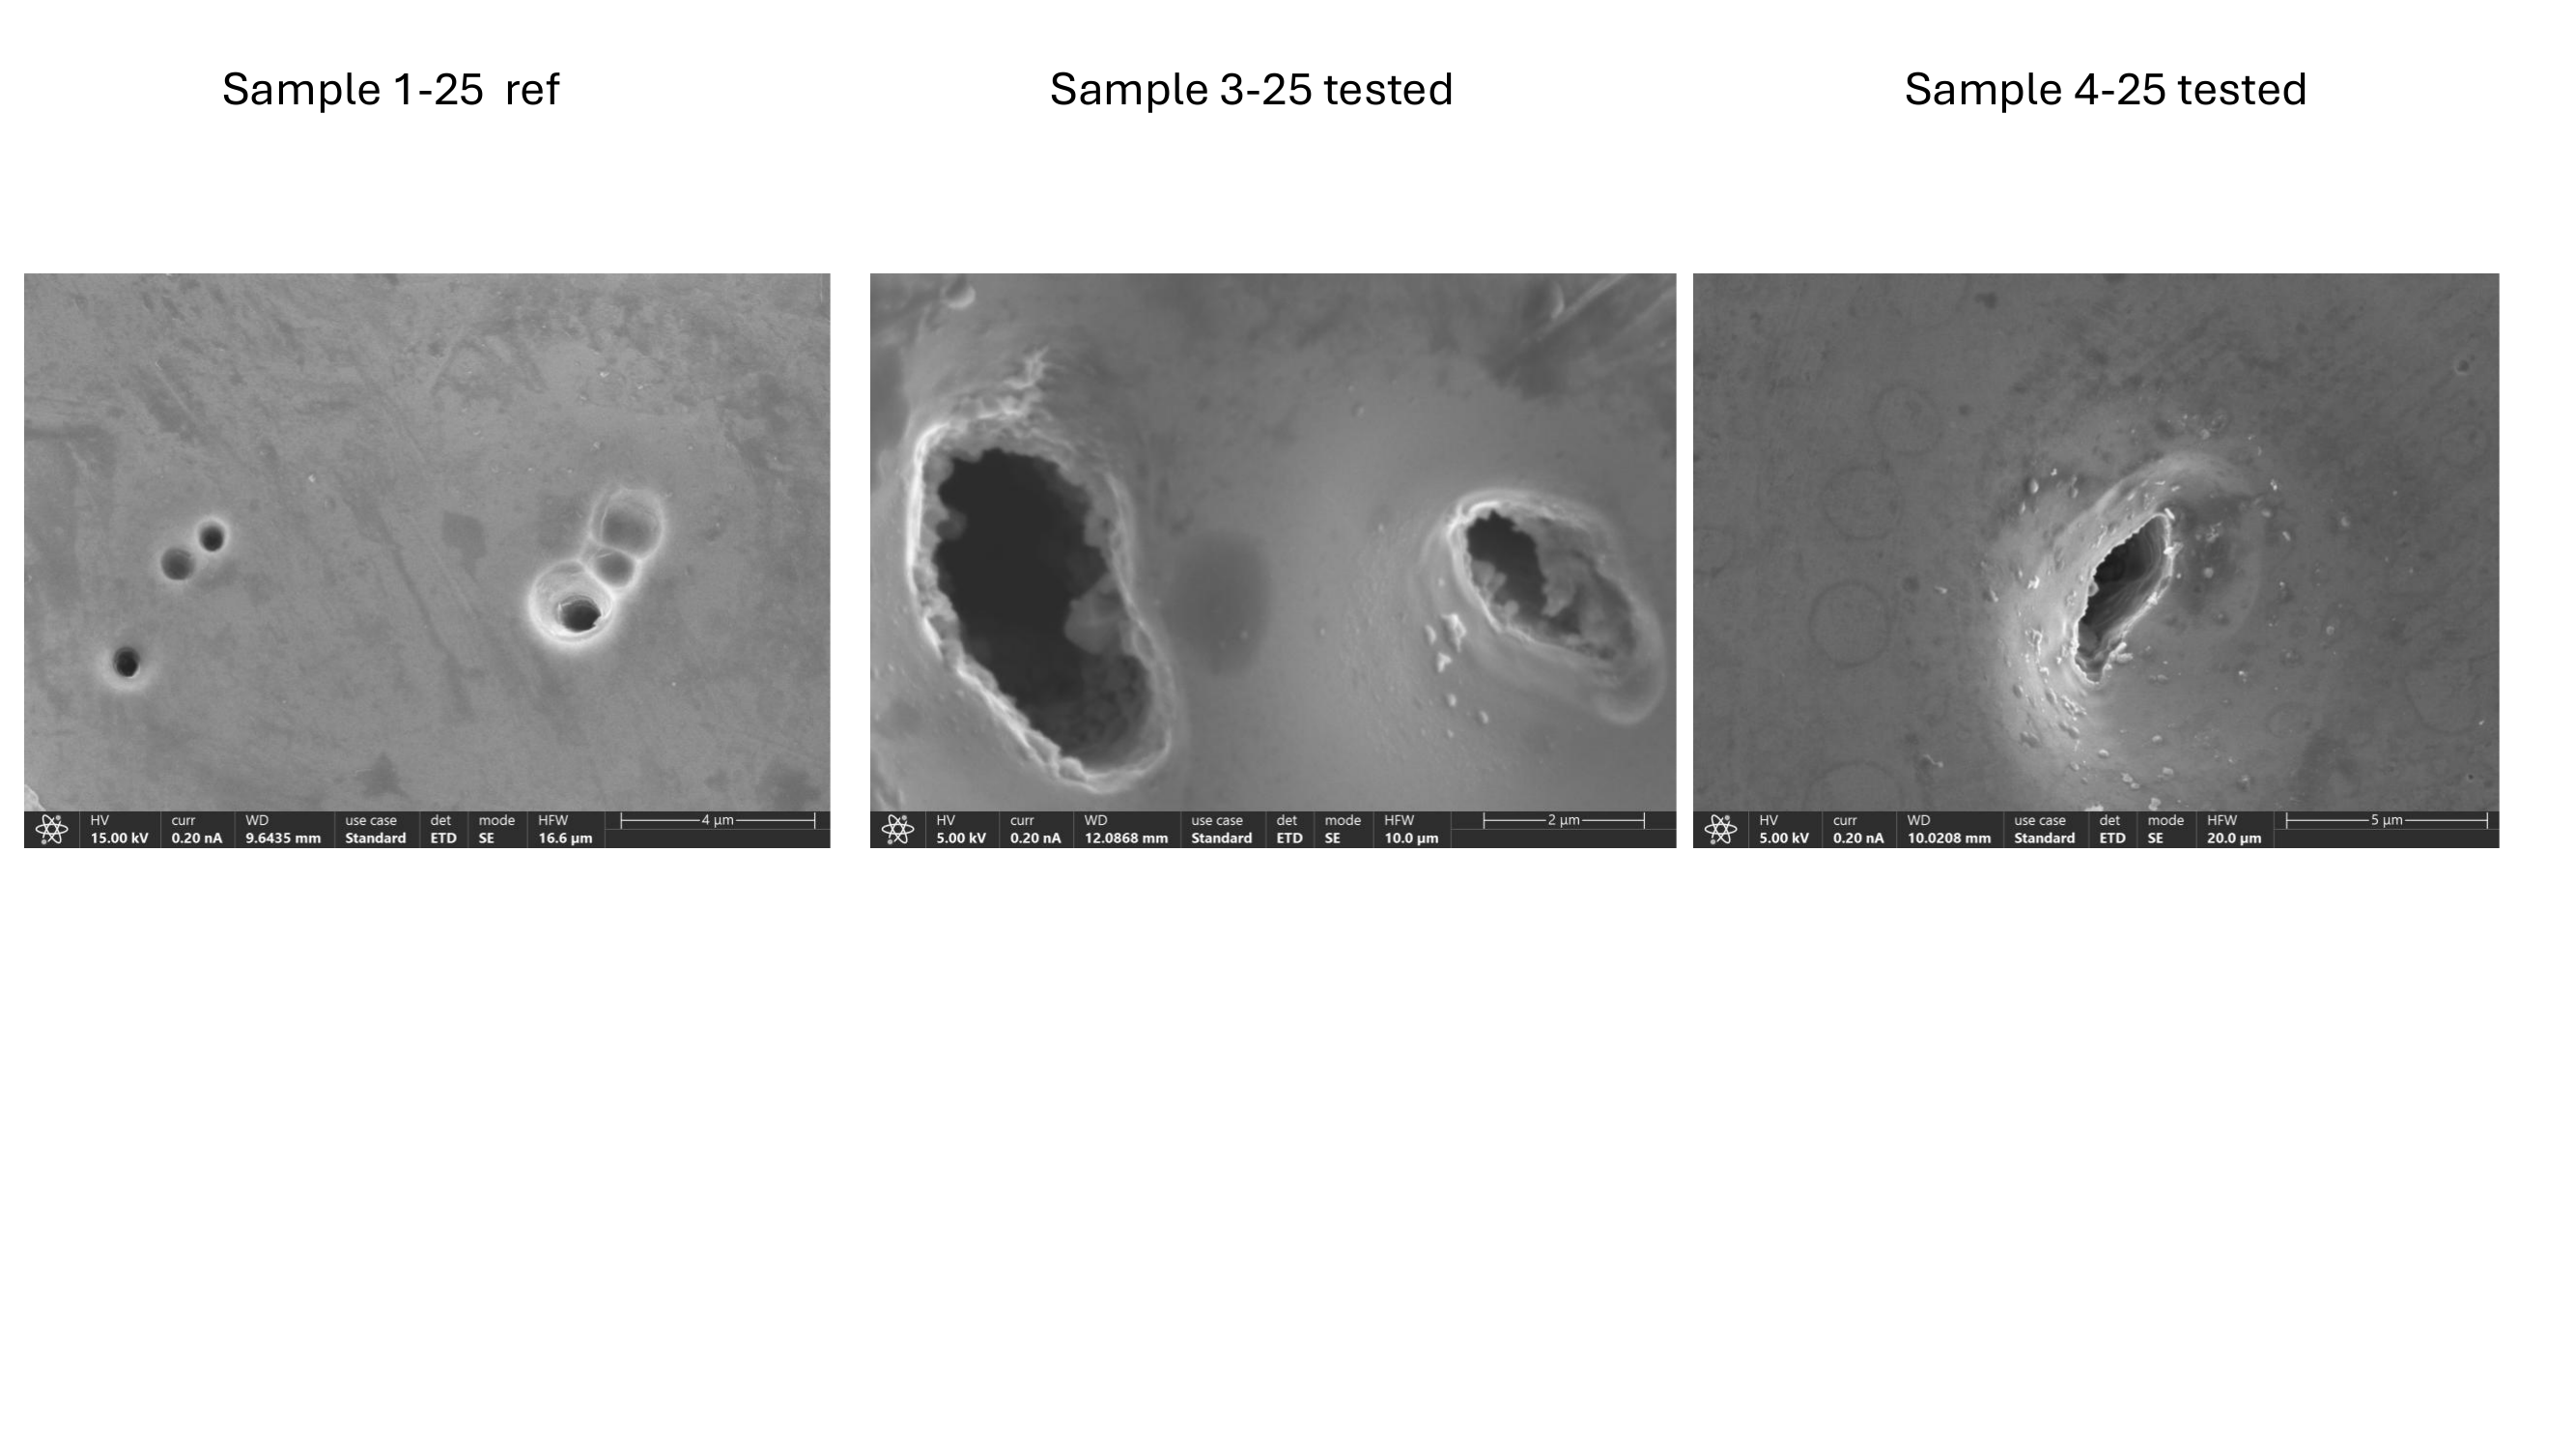
\includegraphics[width=\linewidth]{sem_page-6.png}
    \column{0.27\textwidth}
      \begin{itemize}\setlength\itemsep{0.48em}
        \item Reference: cleaner, rounded cavities
        \item Tested: irregular erupted sites
        \item Typical scale: $1$--$\SI{7}{\micro m}$
        \item No clear molten rim or recast layer
      \end{itemize}
  \end{columns}
  \claim{The morphology is consistent with ruptured near-surface inclusions---not yet proof of a field mechanism.}
  \source{HUJI SEM survey of RFX samples \#1-25, \#3-25, and \#4-25 (May 2026).}
  \note{Be conservative. Chemistry is dominated by elements expected in native 304 inclusion families: Ca, Al, Mg, Si, Mn, Cr, Ti, and V; potassium is a contamination flag and carbon is ambiguous. The eruption morphology lacks the molten rim and recast signature of a conventional arc crater. The decisive test is a FIB cross-section through erupted and intact inclusions, plus a quantitative inclusion census on exposed and reference areas.}
\end{frame}

% 14
\begin{frame}{Early EBSD behavior may already be diagnostic}
  \begin{columns}[T]
    \column{0.48\textwidth}
      \tagbox{good}{Reference \#1-25}
      \begin{itemize}\setlength\itemsep{0.45em}
        \item good diffraction patterns
        \item LAM and grain statistics extracted
        \item Cu analysis pipeline transfers
      \end{itemize}
    \column{0.48\textwidth}
      \tagbox{warn}{Field-exposed \#4-25}
      \begin{itemize}\setlength\itemsep{0.45em}
        \item poor pattern quality
        \item higher current / longer exposure did not recover it
        \item cause is unresolved
      \end{itemize}
  \end{columns}
  \vspace{0.25cm}
  \begin{beamercolorbox}[rounded=true,sep=.25cm]{block body}
    \centering
    \textbf{Three hypotheses:} preparation variation \quad conditioning-induced defects \quad oxide/contamination overlayer
  \end{beamercolorbox}
  \claim{Pattern degradation is evidence only if it repeats and follows the field gradient.}
  \source{RFX project status and HUJI EBSD update, 13 July 2026.}
  \note{This is deliberately framed as an observation, not a result. EBSD information depth is tens of nanometers, so defects or a surface overlayer could degrade pattern quality. A repeat on the second exposed and second reference sample is essential. Quantitative image-quality metrics, hit rate, mean angular deviation, and raw EBSPs should be retained.}
\end{frame}

% 15
\begin{frame}{The decisive comparison is within each exposed hemisphere}
  \centering
  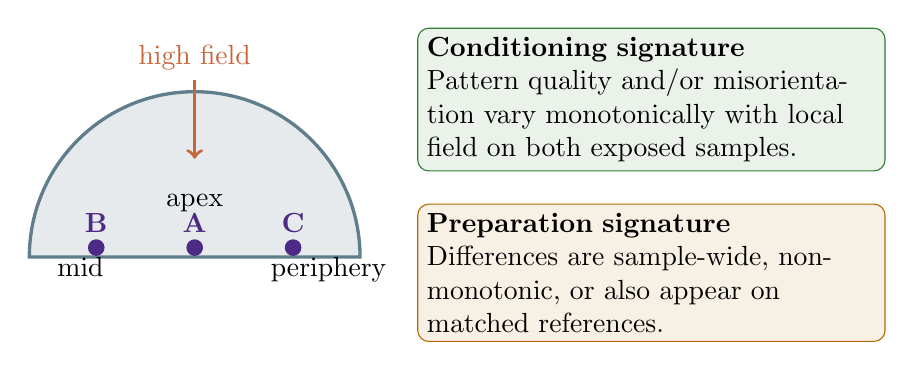
\begin{tikzpicture}[x=1cm,y=1cm]
    \draw[fill=steel!16,draw=steel,very thick] (0,0) arc[start angle=180,end angle=0,radius=2.1cm] -- cycle;
    \draw[->,very thick,copper] (2.1,2.25) -- (2.1,1.25);
    \node[above,copper] at (2.1,2.25) {high field};
    \node[below] at (2.1,.92) {apex};
    \node[below] at (.65,.12) {mid};
    \node[below] at (3.8,.12) {periphery};
    \foreach \x/\lab in {2.1/A,.85/B,3.35/C}{\fill[purple] (\x,.12) circle (3pt); \node[above=2pt,purple] at (\x,.12){\bfseries\lab};}
    \node[draw=good,fill=good!10,rounded corners,align=left,text width=5.7cm] at (7.9,2.00) {\textbf{Conditioning signature}\\Pattern quality and/or misorientation vary monotonically with local field on both exposed samples.};
    \node[draw=warn,fill=warn!10,rounded corners,align=left,text width=5.7cm] at (7.9,-0.20) {\textbf{Preparation signature}\\Differences are sample-wide, non-monotonic, or also appear on matched references.};
  \end{tikzpicture}
  \vspace{0.35cm}
  \claim{The gradient converts an ambiguous sample contrast into a falsifiable spatial prediction.}
  \note{Lay out the measurement matrix: apex, mid-latitude, and periphery on both exposed electrodes, with matched positions on both references. Add EDS carbon/oxygen checks to separate defect density from an overlayer. Correlate quantitative EBSD pattern-quality metrics first; only compare LAM/KAM where indexing quality is adequate and controlled.}
\end{frame}

% 16
\begin{frame}{Depth profiling can manufacture the signal we seek}
  \begin{columns}[T]
    \column{0.31\textwidth}
      \tagbox{warn}{Ga damage}
      \vspace{0.2cm}
      {\small A $\SI{30}{kV}$ FIB can damage a layer comparable to the EBSD information depth.}
    \column{0.31\textwidth}
      \tagbox{warn}{Redeposition}
      \vspace{0.2cm}
      {\small Serial milling can mix material and obscure the true depth coordinate.}
    \column{0.31\textwidth}
      \tagbox{warn}{False martensite}
      \vspace{0.2cm}
      {\small Ion irradiation can transform metastable austenite to BCC, mimicking $\alpha'$ formation.}
  \end{columns}
  \vspace{0.45cm}
  \begin{beamercolorbox}[rounded=true,sep=.28cm]{block body}
    \textbf{Pilot-first control:} identical preparation on exposed and reference material; low-energy final polish; dose bookkeeping; go/no-go before the full $\sim\SI{1}{\micro m}$ campaign.
  \end{beamercolorbox}
  \claim{Preparation artifacts are part of the experiment, not a post-processing detail.}
  \source{RFX artifact review; Babu et al., Acta Mater. 120, 391 (2016).}
  \note{This is the main technical risk. A ten-nanometer serial step is not physically meaningful if the ion-damaged layer is 20--30 nm and the EBSD signal depth is 20--50 nm. Metastable austenite adds a special hazard: Ga or Xe irradiation can generate BCC material with orientation relations that look like deformation martensite. The pilot must establish the artifact floor on a reference before any phase-change claim.}
\end{frame}

% 17
\begin{frame}{Every outcome constrains the conditioning mechanism}
  \begin{columns}[T]
    \column{0.32\textwidth}
      \begin{beamercolorbox}[rounded=true,sep=.24cm]{block body}
        \centering\bfseries\color{good} SS tracks field\\[0.18cm]
        \normalfont\small Supports a cross-material structural state despite different slip physics and loading.
      \end{beamercolorbox}
    \column{0.32\textwidth}
      \begin{beamercolorbox}[rounded=true,sep=.24cm]{block body}
        \centering\bfseries\color{purple} SS changes differently\\[0.18cm]
        \normalfont\small Separates material-specific carriers: planar slip, twins, phase change, or inclusions.
      \end{beamercolorbox}
    \column{0.32\textwidth}
      \begin{beamercolorbox}[rounded=true,sep=.24cm]{block body}
        \centering\bfseries\color{warn} No resolved change\\[0.18cm]
        \normalfont\small Bounds the accessible depth, dose, and sensitivity of dislocation-based models.
      \end{beamercolorbox}
  \end{columns}
  \vspace{0.55cm}
  \claim{The next result is not simply “positive or negative”; it is a mechanism discriminator.}
  \note{This slide is the payoff for presenting RFX as a future direction. A positive correlation supports generality. A qualitatively different response can identify which material degrees of freedom store the state. A null result, if exposure and measurement sensitivity are quantified, places a useful bound and may distinguish cyclic from continuous loading.}
\end{frame}

% 18
\begin{frame}{Conditioning appears to leave a subsurface memory}
  \begin{columns}[c]
    \column{0.54\textwidth}
      \begin{enumerate}\setlength\itemsep{0.55em}
        \item In copper, large-area misorientation is ${\sim}75\%$ higher in high-field regions.
        \item Its spatial hierarchy follows the conditioning-state profile $E_S$.
        \item Stainless steel tests whether that memory survives a change of alloy and loading mode.
      \end{enumerate}
    \column{0.42\textwidth}
      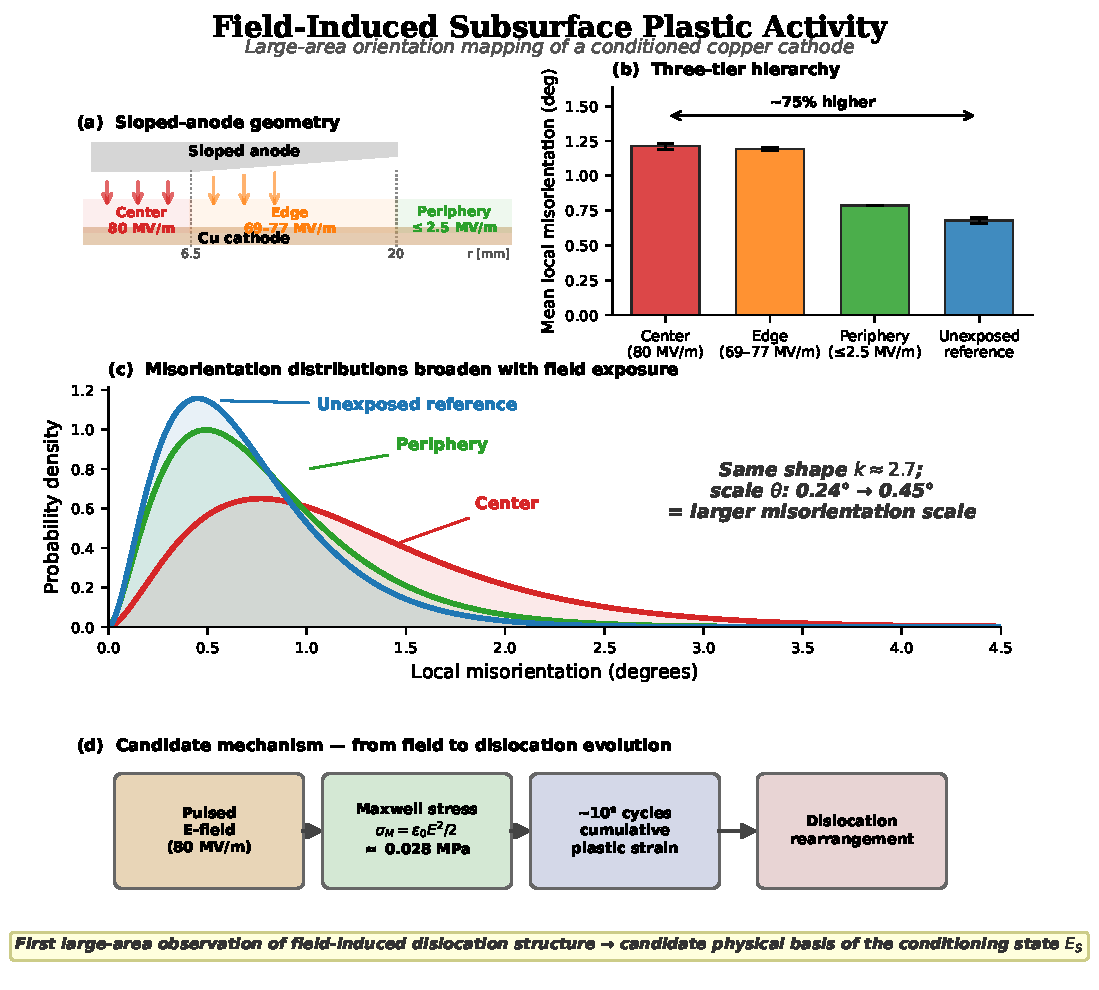
\includegraphics[width=\linewidth]{infographic.pdf}
  \end{columns}
  \vspace{0.25cm}
  \begin{beamercolorbox}[rounded=true,sep=.28cm]{block body}
    \centering\Large\bfseries\color{purple}
    We can now ask what conditioning stores---and where it stores it.
  \end{beamercolorbox}
  \note{Return to the opening question. The copper data provide a measurable structural memory correlated with field exposure and the modeled conditioning state. The RFX experiment is designed to falsify or generalize that interpretation. End on the two coordinates now accessible: lateral field gradients and depth-resolved structure. Invite discussion about the most discriminating SS measurements and the connection to operational conditioning models.}
\end{frame}

\appendix
\begin{frame}{Backup: RFX sample and data status}
  \small
  \begin{tabular}{@{}llll@{}}
    \toprule
    Sample & Role & Surface & Current status \\
    \midrule
    \#1-25 & reference & electropolished & SEM + good EBSD \\
    \#2-25 & reference & electropolished & follow-up acquisition planned \\
    \#3-25 & field-exposed & $\geq\SI{100}{h}$ HV & SEM; EBSD follow-up \\
    \#4-25 & field-exposed & $\geq\SI{100}{h}$ HV & SEM; poor initial EBSD \\
    \bottomrule
  \end{tabular}
  \vspace{0.55cm}
  \begin{itemize}
    \item Outstanding: full conditioning report; numerical $E(\theta)$ vector; alloy certificate; electropolishing protocol.
    \item Needed for interpretation: quantitative EBSD quality metrics and raw patterns; matched EDS overlayer checks.
  \end{itemize}
  \note{Use only if asked about readiness or missing inputs. This status reflects the written project record through 13 July 2026.}
\end{frame}

\begin{frame}{Backup: copper result in one figure}
  \centering
  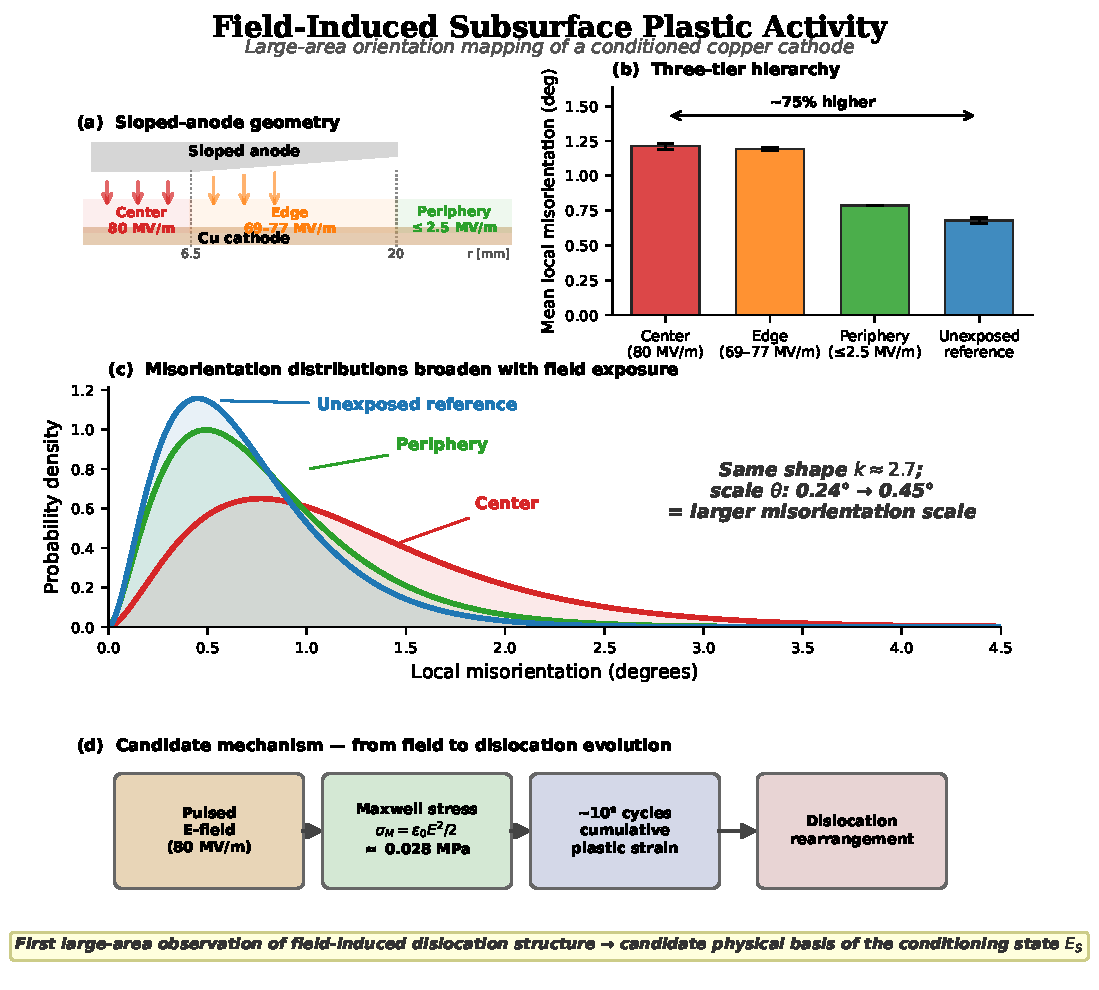
\includegraphics[height=6.55cm]{infographic.pdf}
  \note{Use this as a compact answer to questions about geometry, distributions, or the proposed conditioning mechanism.}
\end{frame}

\end{document}
